\documentclass{article}
\usepackage[utf8]{inputenc}

\usepackage{amsmath,amssymb,amsfonts,bm}
\usepackage{scalerel}
\usepackage{mathtools}
\usepackage{graphicx}
\usepackage{float}
\usepackage{mathrsfs}
\usepackage{hyperref}
\usepackage{subcaption}

\usepackage[
    style=apa,
    backend=biber,
    sortcites=true,
    sorting=nyt,
%    isbn=false,
%    url=false,
%    doi=false,
%    eprint=false,
    hyperref=false,
    backref=false,
%    firstinits=false,
]{biblatex}

\bibliography{Proposal/proposal-refs}

\title{IQP Proposal: Digitization and Mapping of Named Erratics via ArcGIS}
\author{Ethan Chandler}
\date{}

\begin{document}

\maketitle

\section{Introduction}
Glacial erratics, large boulders, and rock fragments transported and deposited by ice sheets far from their original locations are an important part of North American geological and cultural history. Many of these erratics have been recognized for their geological significance \cite{DARWIN1842, Bond1992, Evenson2009}, cultural narratives \cite{Hutton2013}, or even as local landmarks \cite{Hoyt1971}. Among these, certain erratics have been given proper names by local communities \cite{Martin2019}, indicating their importance not only as geophysical markers but also as nodes in the cultural landscape. These named erratics are sites of varying ranges of significance, acting as symbols of reverence \cite{Hellerstein2007}, meeting places, territorial markers, or even travel landmarks. Mapping these named erratics can offer insights into cultural patterns and historical narratives of the 19th and 20th centuries.

This IQP aims to transform a previously hand-drawn map of named erratics \cite{Hutton2012} across North America into a digitized, georeferenced resource using ArcGIS \cite{ESRI2011}. This effort will integrate humanities perspectives with spatial analysis, providing researchers and the public alike with a dynamic digital map of named erratics. The resulting dataset and map will serve as a foundation for future research into the cultural, historical, and geological dimensions of these erratics.

\section{Literature Review}
The study of glacial erratics crosses disciplinary boundaries. From a geological standpoint, erratics have long been studied to understand past glacial extents, ice-flow directions, and the timing of glacial retreat \cite{DARWIN1842, Bond1992, Evenson2009, Colgan2009, Clark2018, Emery2023}. Beyond geology, erratics have also attracted the attention of cultural geographers and humanists, as they sometimes hold spiritual \cite{Delabarre1928, Hutton2013}, aesthetic, or historical significance \cite{Hellerstein2007}. These stones can be found embedded in Indigenous meeting places \cite{Hutton2013}, colonial travel narratives, or local folklore, functioning as anchors that bear witness to human-environment interactions. 

\begin{figure}[H]
    \centering
    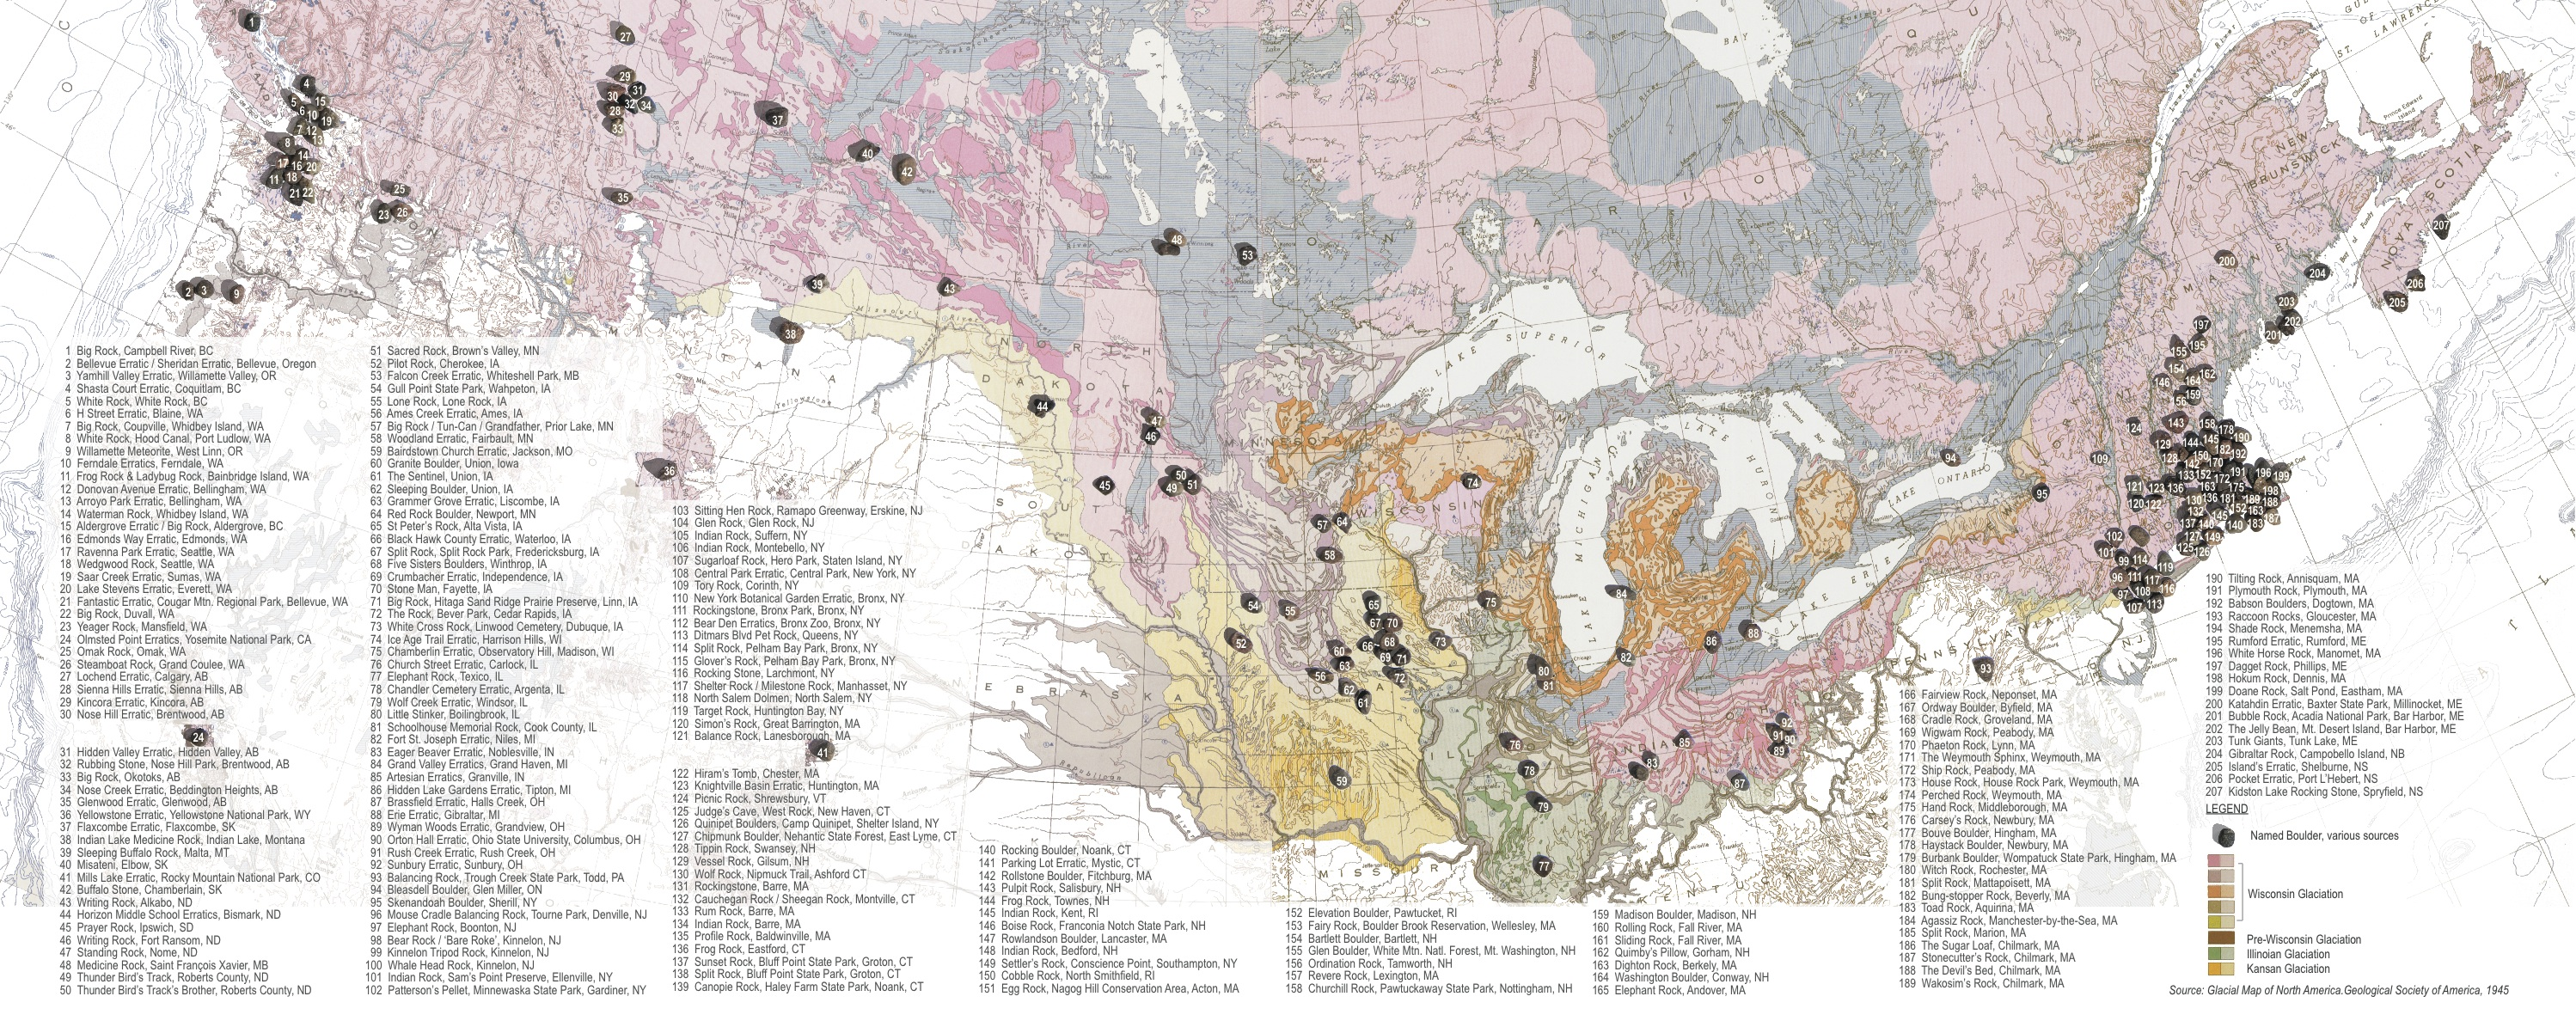
\includegraphics[width=0.95\textwidth]{Images/JanesMap.jpg}
    \caption{Original static map \cite{Hutton2012}.}
    \label{fig:original_map}
\end{figure}

\begin{figure}[H]
    \centering
    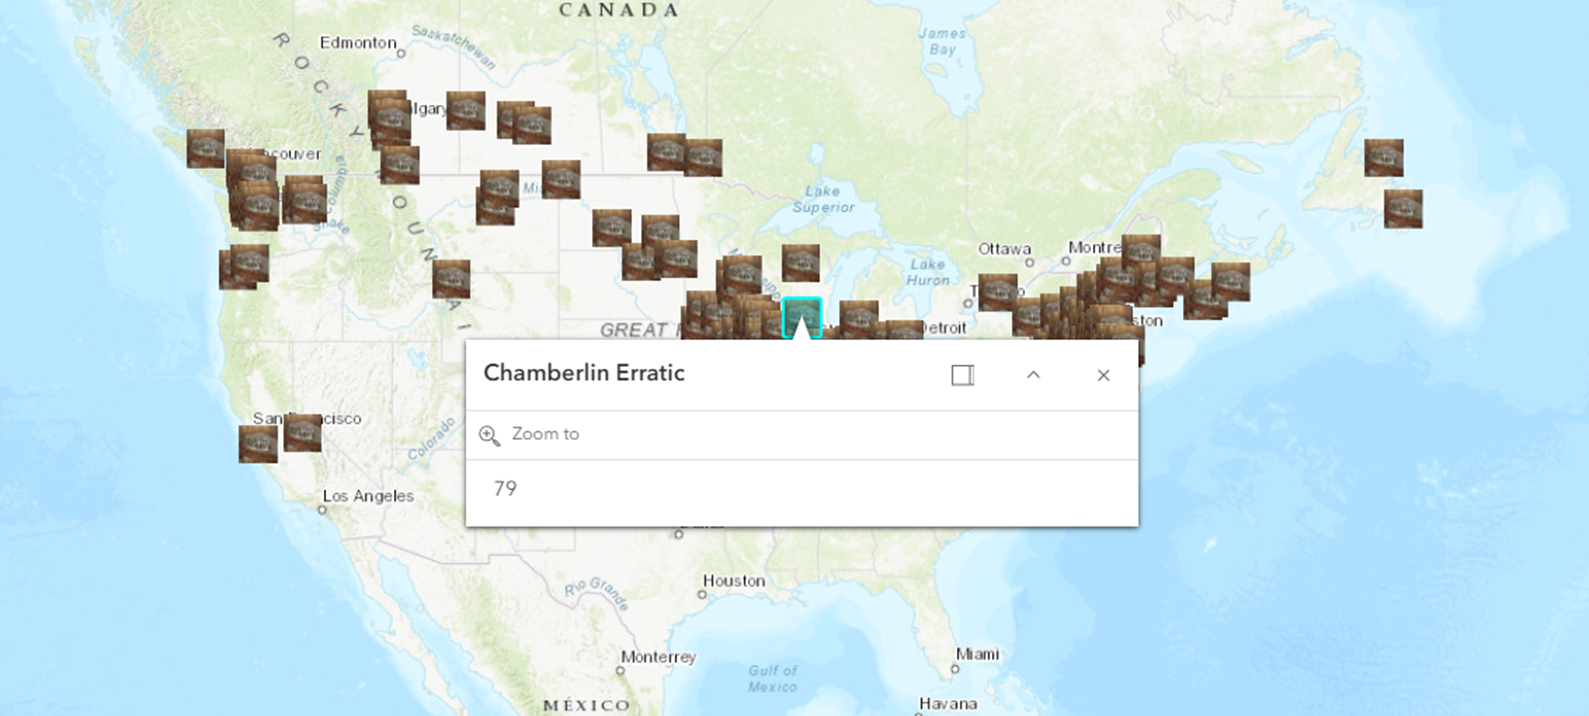
\includegraphics[width=0.95\textwidth]{Images/DigitizedMap.png}
    \caption{Dynamic map prototype.}
    \label{fig:prototype}
\end{figure}

This literature review is broken down into three subsections. Section \ref{sec:Geological} discusses the geological significance of erratics from a scientific perspective, Section \ref{sec:Cultural} details the cultural significance of specific named erratics through a series of case studies, and Section \ref{sec:GIS} provides a brief background on Geographical Information Systems (GIS).

\subsection{Geological Considerations}\label{sec:Geological}
From a geological perspective, erratics are key indicators of past glacial dynamics. The lithological composition and spatial attributes of erratics can provide clues about the direction of ice flow, the provenance of bedrock sources, and the extent of ice sheets during the Pleistocene \cite{Bond1992, Evenson2009, Clark2018}.\footnote{The Pleistocene is a geological time period that lasted roughly from 2.58 million to 11,700 years ago, and is colloquially known as the last Ice Age.} For instance, matching the composition of an erratic to a known bedrock source region can help reconstruct the trajectories of glacial lobes and identify patterns of subglacial transport \cite{Colgan2009, Emery2023}. Erratics have therefore served as critical evidence in debates over glacial theory since the early works of geologists like Darwin, who noted their distribution and potential significance for understanding past climates and earth surface processes \cite{DARWIN1842}.

Beyond mapping ice-flow directions, erratics help constrain the timing of glaciation and deglaciation. Cosmogenic nuclide dating techniques applied to large erratics have refined our understanding of ice margin retreat rates, particularly in North America \cite{Colgan2009, Clark2018}.\footnote{Cosmogenic nuclide dating---a common method of surface exposure dating in literature---is a geochronological dating technique which measures the concentration of certain particles dislodged from cosmic rays in order to find how long a certain piece of material as been buried.} Furthermore, the presence of erratics in unexpected locations---at high elevations, far into lowland areas, or perched in precarious positions---can challenge and refine existing glacial models.

\subsection{Cultural and Historic Signifigance}\label{sec:Cultural}
The cultural significance of erratics emerges from their stable, enduring presence on the landscape. While their geological journey ended thousands of years ago, their cultural histories often began at contact with human communities. In many cases, erratics became landmarks for navigation, meeting places for ceremonies, or even objects of reverence \cite{Hellerstein2007, Delabarre1928}. Oral histories \cite{Hoyt1971}, indigenous traditions, and colonial travel writings frequently highlight these stones as meaningful points in the environment---both physically and symbolically.

Named erratics, in particular, stand at the intersection of geological time and human narrative. They have acquired names through repeated social engagement, functioning as cultural anchors in a shifting historical terrain \cite{Hutton2013, Martin2019}. Over time, these named erratics have been integrated into local myths and municipal identities. They represent sites where history and geological heritage intertwine, making them interesting subjects for interdisciplinary study.
\subsubsection{Case Studies}
\paragraph{Dighton Rock}
Dighton Rock, located in the Taunton River in Massachusetts, exemplifies the complex interplay between natural history and cultural narrative. This sandstone boulder is covered with petroglyphs whose origin has been debated for centuries, attributed variously to indigenous peoples, early European explorers, or even more speculative sources \cite{Delabarre1928}. While geologically unremarkable as an erratic, its cultural inscriptions have transformed it into a contested artifact of human history. Over time, Dighton Rock has been studied by antiquarians and archaeologists alike, who have sought to decode its carvings---making it a prime example of an erratic that transcends its geological roots to become a cultural and historical enigma.

\paragraph{Plymouth Rock}
Plymouth Rock, arguably one of North America’s most famous named erratics, is traditionally identified as the landing site of the Pilgrims in 1620. Although geologists recognize it as a locally sourced boulder moved by glacial action, its cultural narrative outshines its geological significance. As a symbol of American heritage, it features prominently in school curricula and national narratives \cite{Hellerstein2007}. The rock’s preservation and curation in a designated monument underscore how an erratic can become not only a historic waypoint but an enduring national symbol.

\paragraph{Babson's Boulders}
In the former colonial settlement of Dogtown, Massachusetts, entrepreneur and philanthropist Roger Babson commissioned the carving of motivational inscriptions on dozens of glacial erratics scattered throughout the abandoned town site. Known collectively as Babson’s Boulders, these erratics bear words such as “Courage,” “Integrity,” and “Kindness.” While geologically, these are standard granitic glacial erratics, culturally, they form a scenery of text-mediated values \cite{Hutton2013, Martin2019}. The stones exemplify how erratics can be re-inscribed with meaning through direct human intervention, transforming them into a didactic landscape that reflects the social and moral aspirations of a community at a given historical moment.

\paragraph{Rollstone Boulder}
The Rollstone Boulder, originally perched atop Rollstone Hill in Fitchburg, Massachusetts, was a prominent landmark noted for its imposing size and prominent visibility. Recognized by local inhabitants and travelers alike, it eventually became a civic symbol. The residents of Fitchburg had become so attached to their intrepid boulder that they cemented the joints and bound Rollstone Boulder with an iron band \cite{Fitchburg1908} to protect it from rolling into the hillside river. Additionally, when quarrying threatened its original resting place, the citizens of Fitchburg had it disassembled, moved, and reassembled in the city center in 1929 \cite{Fitchburg1908}. Through this relocation, the town effectively “rescued” its erratic from geological obscurity, re-situating it as a central cultural monument. Rollstone Boulder’s transition from a glacial remnant to an urban heritage icon exemplifies how communities can actively preserve and redefine the meaning of named erratics. These acts of protection and attachment to an otherwise benign boulder emphasize the personal connection people felt to these mighty rocks.

\subsection{Geographic Information Systems (GIS)}\label{sec:GIS}
Recent advances in Geographic Information Systems (GIS) \cite{Elghazaly2023} and digital humanities methods have enabled the spatial humanities to grow rapidly. GIS technologies allow scholars to integrate diverse datasets—such as folklore archives, historical maps, oral histories, and environmental data—into layered, interactive environments \cite{Mennecke1996, ESRI2011, Butler2016}. This approach helps uncover spatial patterns in humanities data that might otherwise go unnoticed. Although some studies have employed GIS to visualize geospatial distributions of cultural artifacts (e.g., historical markers, locations of conflicts) \cite{BennettMaitlandGilgenbachPeasha2017, McKeenFiddes2021}, there is a relative scarcity of studies focusing on digital mapping and spatial analysis of named erratics.

By digitizing and georeferencing Hutton's map of named glacial erratics \cite{Hutton2012}, this project will build upon digital humanities methodologies to reveal the underlying spatial relationships and cultural contexts of these geological features. It will also provide a methodological template for integrating analog, humanistic data into digital mapping platforms.

\section{Research Questions}
This project is guided by the following research questions:

\begin{enumerate}
    \item \textbf{Methodological Insights:} How can GIS methodologies and digital humanities techniques be combined effectively to transform legacy, analog data (e.g., hand-drawn maps) into accessible, analyzable digital resources? Challenges include ensuring data accuracy during digitization, preserving the contextual integrity of the original maps, and managing the integration of diverse datasets with varying levels of sparsity and fidelity. See Section \ref{sec:DataAcquisition}.

    \item \textbf{Function-Based Categorization}
    Is it possible to classify named erratics into functional categories—such as ceremonial sites, territorial markers, or travel waypoints---and what data-driven techniques can best reveal these underlying functional distinctions?\footnote{At present, embedding-based clustering methods seem the most general and scalable. They are well suited for this task because they excel at solving clustering problems with sparse or inaccurate information, such as human literature.} See Section \ref{sec:SpatialAnalysis}.

    \item \textbf{Temporal and Thematic Grouping}
    Do erratics mentioned in earlier (18th–19th century) documents cluster into different thematic categories (e.g., spiritual, folkloric), than those highlighted in 20th-century (e.g., geological, scientific) works and how might these categories reflect shifts in cultural perception over time? What about spatial thematic connections, rather than temporal ones? See Section \ref{sec:SpatialAnalysis}.
\end{enumerate}

\section{Methodology}
This IQP will employ a three-phase methodology over B, C, and D term.

\subsection{B-Term: Data Acquisition, Literature Review, \& Preparation}\label{sec:DataAcquisition}
\begin{enumerate}
    \item \textbf{Source Materials:} Begin with the original map of named glacial erratics in the United States from Hutton \cite{Hutton2012}. Obtain the list of named erratics and the associated GPS data used to create the original map.

    \item \textbf{Literature Review:} Perform a comprehensive literature review of glacial erratics, from both a geological and cultural/historical standpoint. Familiarize with GIS software.

    \item \textbf{Ancillary Data:} Gather supplementary data (e.g., historical context, images, size, topographic region, etc.) for the erratics. Access AAS resources and digital resources to add to the data set in the form of a CSV file.

    \item \textbf{Data Cleaning:} Standardize erratic names and get a sense of the accuracy of the coordinates by cross-referencing with known geological and topographical references.
\end{enumerate}

\subsection{C-Term: Spatial Analysis \& GIS Data Visualization}\label{sec:SpatialAnalysis}
\begin{enumerate}
    \item \textbf{Spatial Analysis:} Conduct analyses to determine patterns in erratic distribution (for instance: Relationships to glacial formations, proximity to colonial and indigenous development, and historical travel routes, military fort locations) to see what stories the data tells. One potential avenue for this is to use embedding-based clustering (Word2Vec, Doc2Vec, Sentence Transformers, etc.). The way it works is we would encode textual descriptions of each erratic into vector embeddings and cluster them using algorithms like DBSCAN \cite{Deng2020} or UMAP \cite{Healy2024}. Erratics that cluster closely might share subtle thematic or historical similarities. For instance, one cluster could consist of erratics that often appear in historical travel guides or early settler diaries. These stones might be repeatedly mentioned as navigational landmarks or notable waypoints on trade or pilgramage routes. Texts would include phrases like ``guidepost", ``direction", or ``mile marker", or references to known roads and rivers. This cluster would fall under the category of ``Navigational Erratics", for instance. This method is basically a way to utilize big data to automatically categorize each erratic into a set of topics, which the user can then toggle on or off on the map.

    \item \textbf{Visualization:} Produce thematic maps showing different aspects of the data (e.g., glacial geology, cultural overlays, terrain layers, military fort locations) in a visually appealing manner. The visualizations should be intuitive enough for national park goers/hikers and K-12 audiences, but accurate and detailed enough for researchers and historians.
\end{enumerate}

\subsection{D-Term: Open-Source Software Release \& Written Analysis}
\begin{enumerate}
    \item \textbf{Public Accessibility:} Publish the resulting GIS layers and digital maps online, potentially incorporating them into an augmented reality (AR) framework (stretch goal). This AR framework could offer users an immersive way to explore the historical and cultural significance of named erratics by overlaying digital content onto physical terrain. The potential impact of an open-source release includes enhanced public engagement, educational applications, and new avenues for crowdsourced research.

    \item \textbf{Evaluation:} Reflect on methodological lessons learned, consider the limitations of the digitization process, and propose directions for future research and improvement---particularly on how this work can be taken up by other project centers. Current ideas include crowdsourcing the process of documenting and uploading named erratics to the map---via an SQL database---and expanding the database to other continents such as South America.
\end{enumerate}

\section{Preliminary Results}
In this section, we discuss the preliminary results of the GIS visualization of the named erratics, based on the dataset used in \cite{Hutton2012}. The code \texttt{GIS-Named-Erratics} is fully open-source and available on \href{https://github.com/echandler5956f/GIS-Named-Erratics}{GitHub}.
Here, we show the programming pipeline for extracting, keying, and rendering each named erratic datapoint:

\begin{figure}[H]
    \centering
    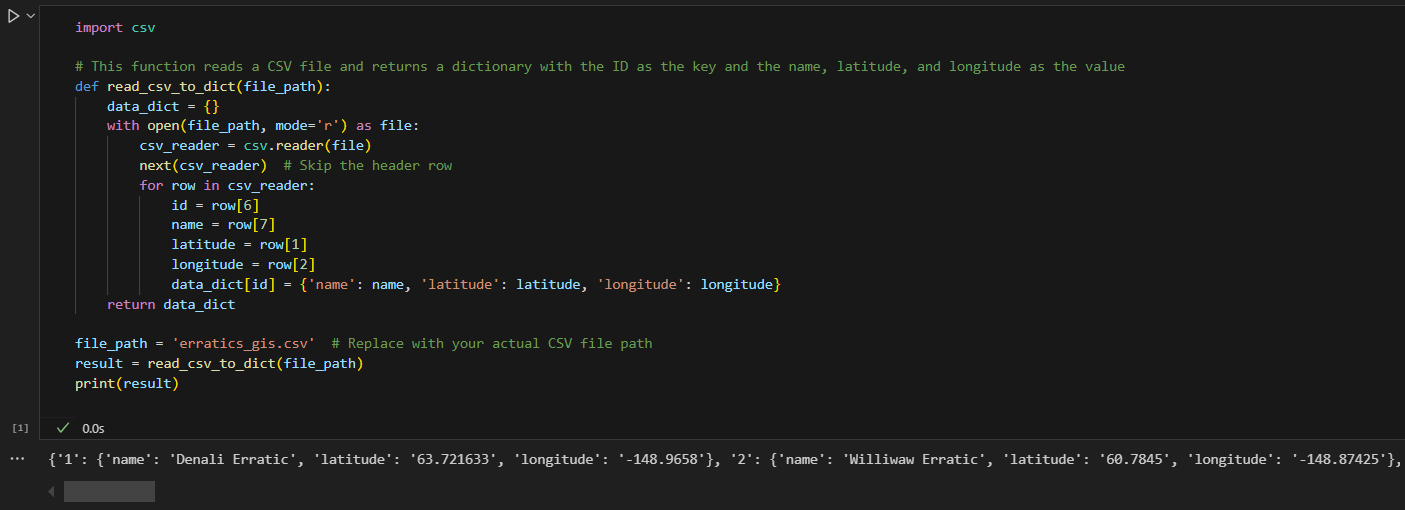
\includegraphics[width=1.0\textwidth]{Images/CodeSnippet1.png}
    \caption{Convert the CSV containing the erratics' metadata into a Python Dictionary.}
    \label{fig:1}
\end{figure}

\begin{figure}[H]
    \centering
    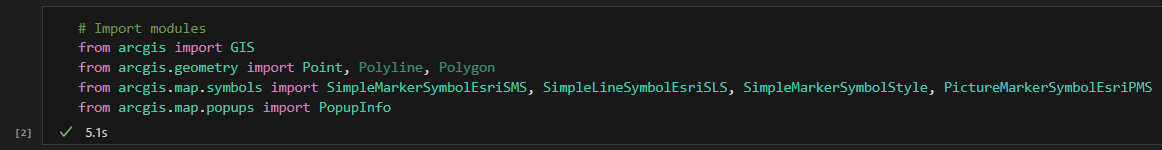
\includegraphics[width=1.0\textwidth]{Images/CodeSnippet2.png}
    \caption{Import necessary \texttt{arcgis} packages.}
    \label{fig:2}
\end{figure}

% \begin{figure}[H]
%     \centering
%     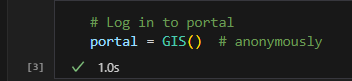
\includegraphics[width=1.0\textwidth]{Images/CodeSnippet3.png}
%     \caption{Log in to \texttt{arcgis}.}
%     \label{fig:3}
% \end{figure}

\begin{figure}[H]
    \centering
    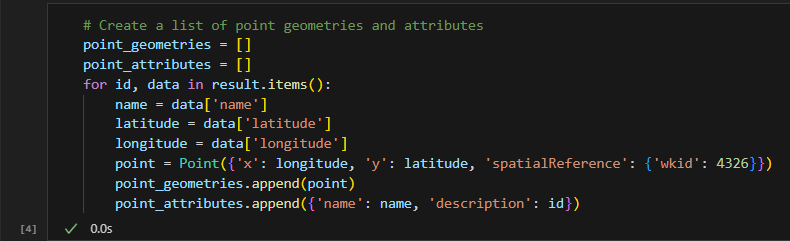
\includegraphics[width=1.0\textwidth]{Images/CodeSnippet4.png}
    \caption{Create a list of \texttt{arcgis} point geometries using the extracted metadata from the CSV.}
    \label{fig:4}
\end{figure}

\begin{figure}[H]
    \centering
    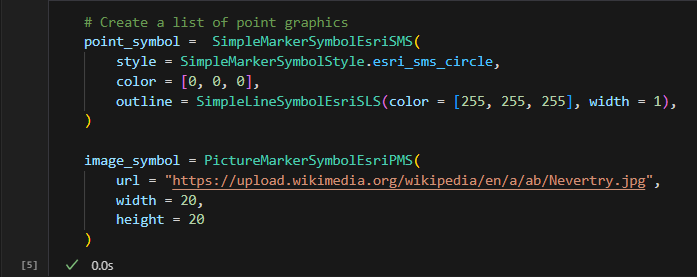
\includegraphics[width=1.0\textwidth]{Images/CodeSnippet5.png}
    \caption{Create the symbols used to render the points with (in the future we will have an image of each individual erratic which we can render, but this code snippet shows how to do it for the simple case of using the same image).}
    \label{fig:5}
\end{figure}

% \begin{figure}[H]
%     \centering
%     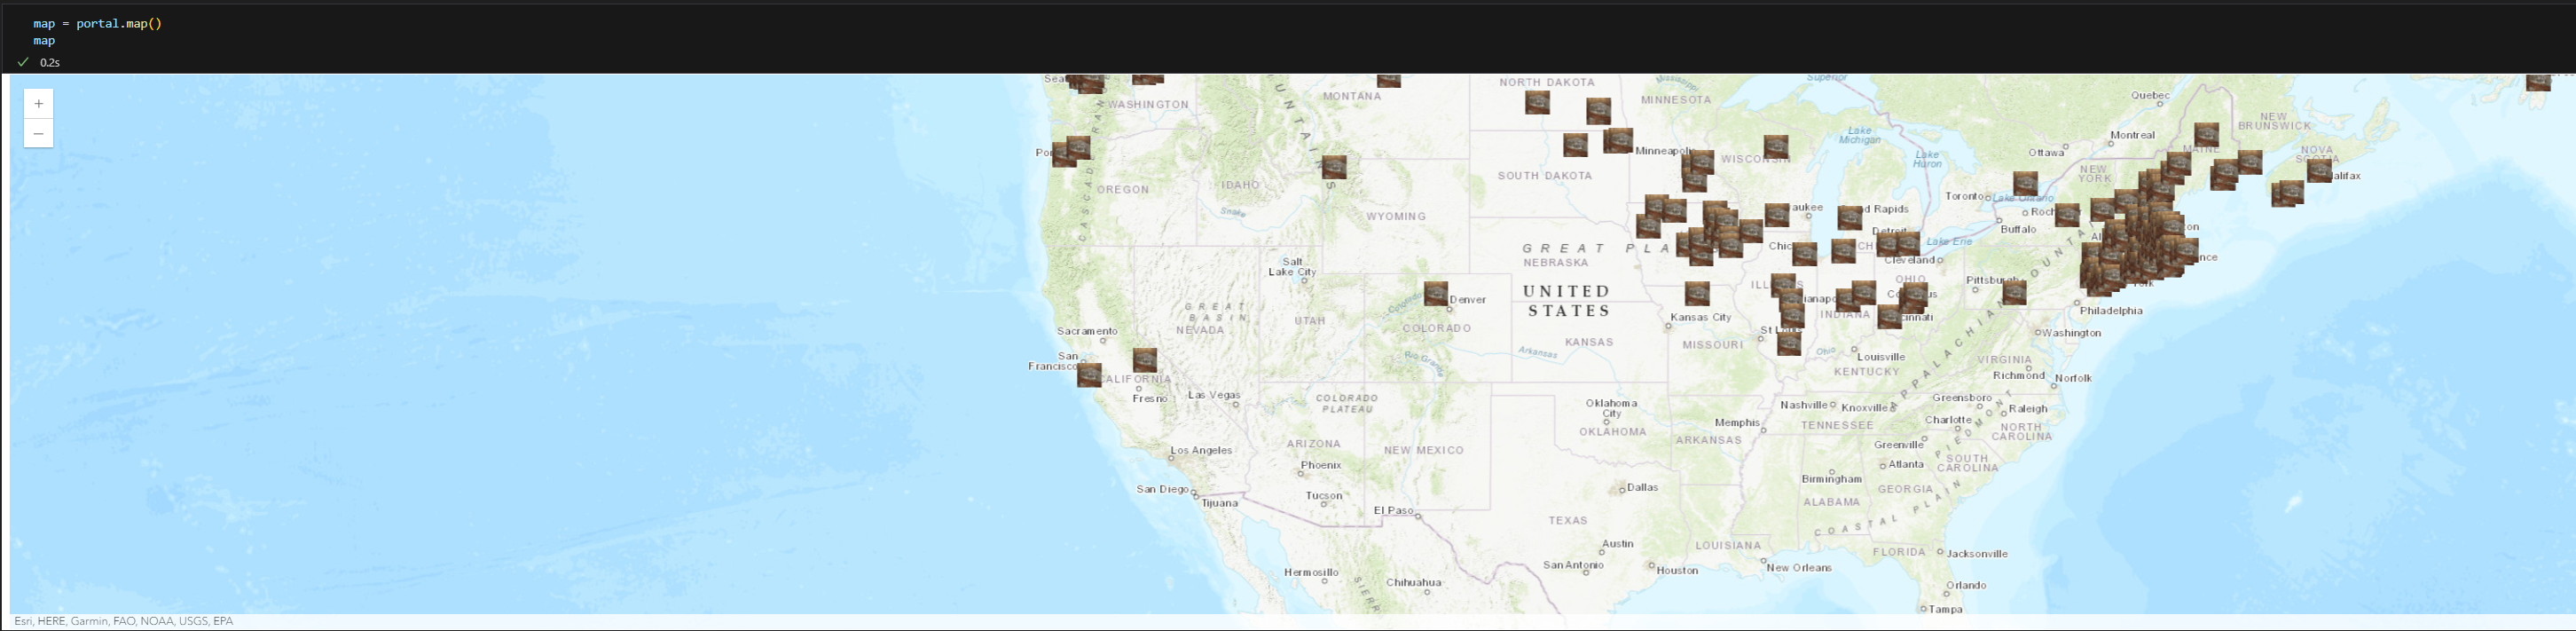
\includegraphics[width=1.0\textwidth]{Images/CodeSnippet6.png}
%     \caption{}
%     \label{fig:6}
% \end{figure}

\begin{figure}[H]
    \centering
    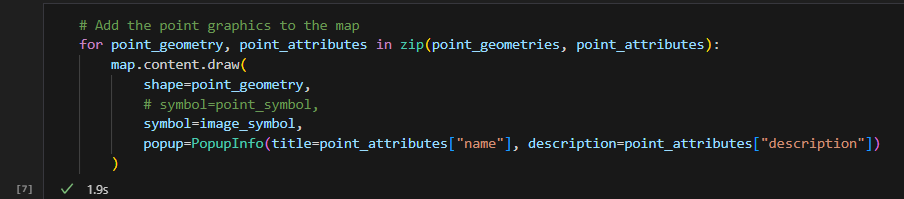
\includegraphics[width=1.0\textwidth]{Images/CodeSnippet7.png}
    \caption{Draw each of the datapoints on the map using, and add a popup box that appears upon clicking the point, which contains a description of the erratic (for now it just shows the erratic ID).}
    \label{fig:7}
\end{figure}

\begin{figure}[H]
    \centering
    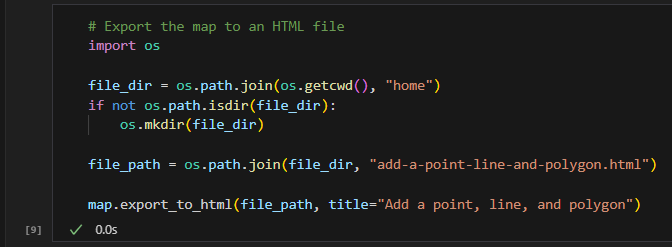
\includegraphics[width=1.0\textwidth]{Images/CodeSnippet9.png}
    \caption{Export the map and save it to an HTML file.}
    \label{fig:9}
\end{figure}

\begin{figure}[H]
    \centering
    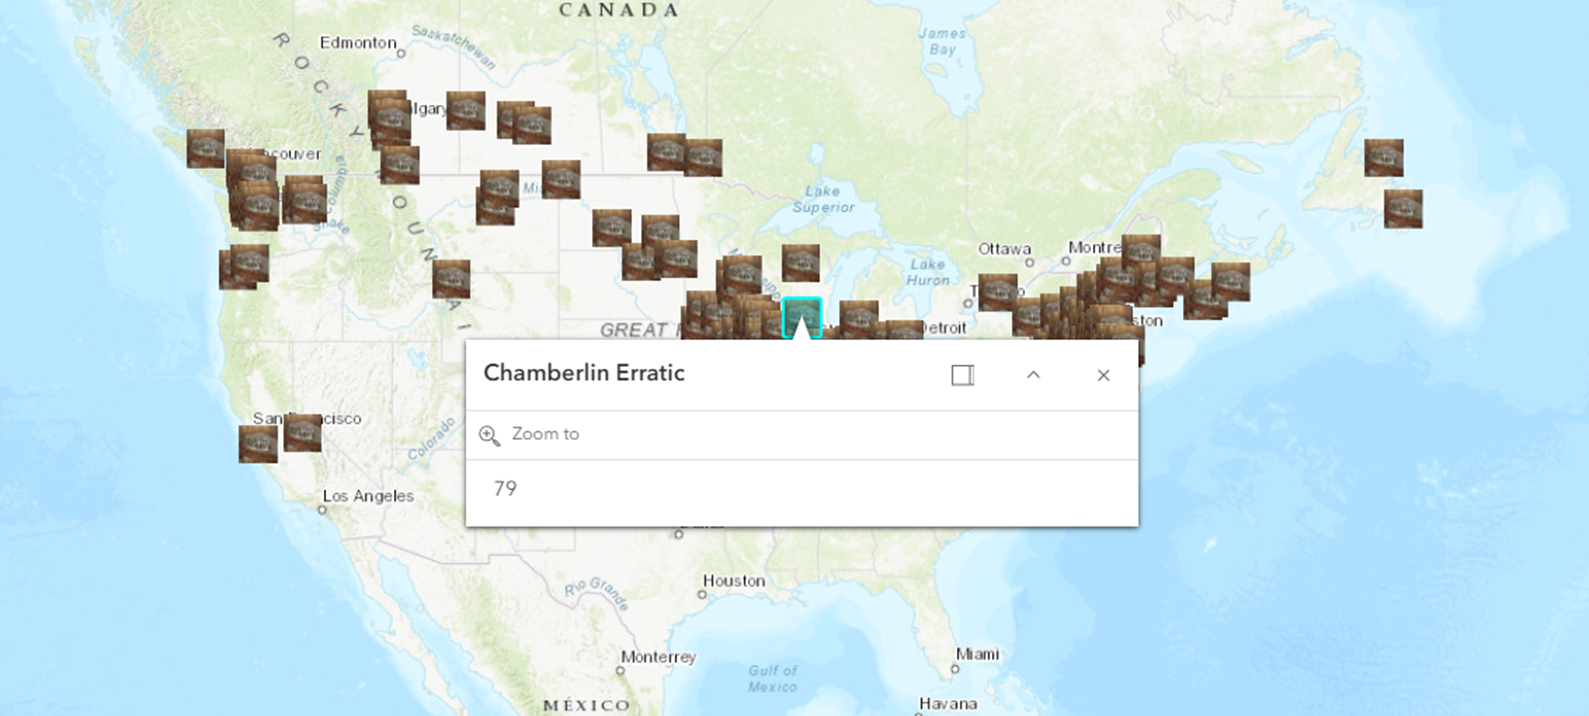
\includegraphics[width=1.0\textwidth]{Images/DigitizedMap.png}
    \caption{Resulting dynamic map.}
    \label{fig:10}
\end{figure}

\section{Conclusion}
By translating a handmade map of named glacial erratics into a digital, GIS-based resource, this project uses spatial humanities to illuminate the intersections of natural and cultural histories. The resulting geospatial dataset and visualizations will enrich our understanding of glacial processes, cultural narratives, and the complex relationships that humans have forged with these ancient rocks. Moreover, the project's methodological approach will provide a model for integrating humanities data with digital mapping platforms, ultimately contributing to more robust, interdisciplinary scholarship.

\section*{Bibliography}
\printbibliography[heading=none]

\end{document}